\documentclass[12pt]{article}
\usepackage[margin=1in]{geometry}
\usepackage{amsmath, amsthm, amssymb, amsfonts, breqn, graphicx}


\theoremstyle{definition}
\newtheorem{problem}{Problem}
\renewcommand*{\proofname}{Solution}
\newenvironment{custompbm}[1]
  {\renewcommand\theproblem{#1}\problem}
  {\endproblem}
\renewcommand{\theenumi}{\alph{enumi}}


\newcommand{\E}{\text{E}}
\newcommand{\V}{\text{Var}}
\newcommand{\Co}[2]{\text{Cov}\left({#1}, {#2}\right)}
\newcommand{\pdf}{\text{pdf}}
\newcommand{\pmf}{\text{pmf}}
\newcommand{\me}{\mathrm{e}}
\newcommand*\diff{\mathop{}\!\mathrm{d}}
\newcommand{\vect}[1]{\boldsymbol{#1}}
\newcommand{\mx}[1][t]{\mu_X({#1})}
\newcommand{\gx}[2]{\gamma_X({#1}, {#2})}


\title{Homework Assignment 10}
\author{Matthew Tiger}


\begin{document}


\maketitle


\begin{problem}
  Plot the energy bills versus time. What kind of trend appears to exist? What type of seasonal
  variation appears to exist? Is a transformation needed to obtain a series that displays constant
  variation?
\end{problem}

\begin{proof}
  See below for a plot of the bills time series data:
  \vskip 0mm
  \begin{center}
  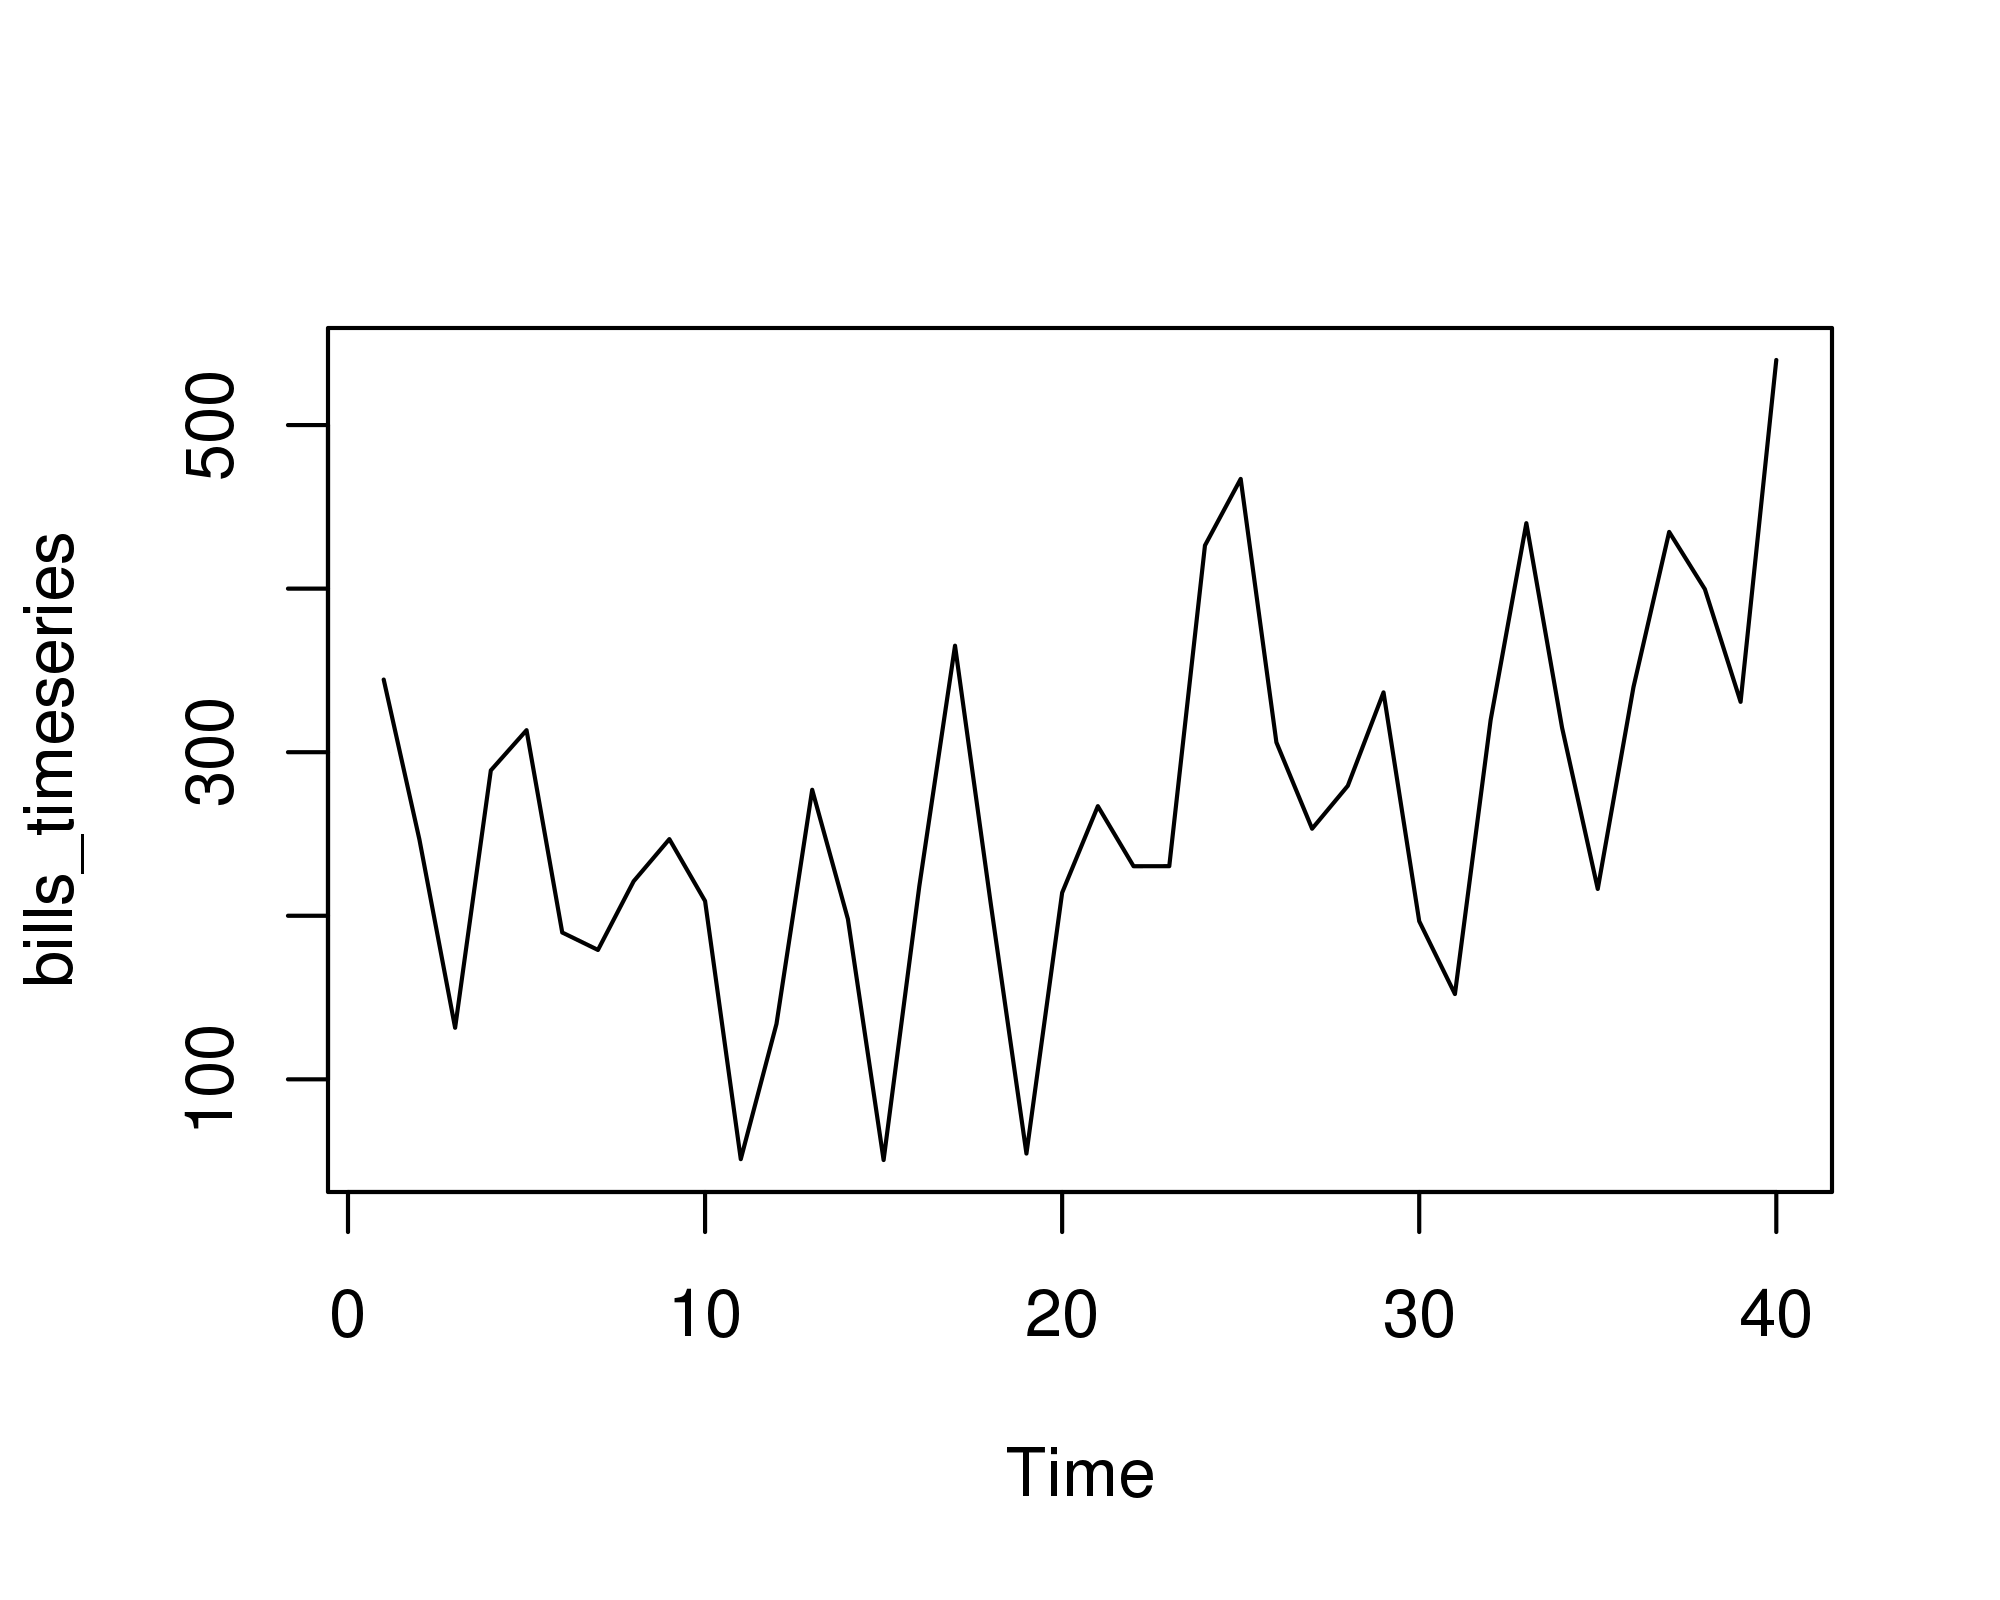
\includegraphics{timeseries}
  \end{center}
  \vskip 10mm

  It is clear from the plot that there is a trend that appears to move upwards
  as time increases and a seasonal variation with period 4
  lags present in the data so a transformation is needed to obtain residuals
  that represent a stationary time series.
\end{proof}


\begin{problem}
  Write algebraically a time series model with trend and seasonal component with definitions
  of the dummy variable.
\end{problem}

\begin{proof}
  Note that it appears that this time series has a quadratic trend. Additionally,
  we are interested in capturing the seasonal quarter data of the time series.
  Therefore, a time series model for the data with trend and seasonal components is given by
  \[
    X_t = a_0 + a_1 t + a_2 t^2 + a_3 Q_1 + a_4 Q_2 + a_5 Q_3 + a_6 Q_4,
  \]
  where we define $Q_i$ as 1 if $t \equiv i \mod 4$ and 0 otherwise and $a_j$ is
  constant.
\end{proof}


\begin{problem}
  Are all the variables in the model statistically significant? Justify your answer.
\end{problem}

\begin{proof}
  The following \texttt{R} code performs a linear regression on our data set using the
  above equation:
  \begin{verbatim}
quarter_variable <- function(ts, position){
    vector <- rep(0, 4)
    vector[position] <- 1

    variable <- rep(vector, length(ts) / 4)

    return(variable)
}

bills <- scan("bills.csv", skip=1)
bills.ts <- ts(bills)

bills.ts.Q1 <- quarter_variable(bills.ts, 1)
bills.ts.Q2 <- quarter_variable(bills.ts, 2)
bills.ts.Q3 <- quarter_variable(bills.ts, 3)
bills.ts.Q4 <- quarter_variable(bills.ts, 4)

bills.ts.regression_equation <- bills.ts ~ 0 + time(bills.ts) +
    I(time(bills.ts)^2) + bills.ts.Q1 + bills.ts.Q2 + bills.ts.Q3 +
    bills.ts.Q4
bills.ts.regression <- lm(bills.ts.regression_equation)

# The following tells us that all variables are significant
# using a significance level of alpha = 0.05.
summary(bills.ts.regression)

  \end{verbatim}

  The code above outputs the following table displaying the significance of the
  variables in the regression equation:
  \begin{verbatim}
Coefficients:
                    Estimate Std. Error t value Pr(>|t|)
time(bills.ts)       -7.4582     3.3960  -2.196 0.034999 *
I(time(bills.ts)^2)   0.3012     0.0803   3.751 0.000657 ***
bills.ts.Q1         342.4070    33.8113  10.127 8.44e-12 ***
bills.ts.Q2         238.7662    34.3165   6.958 5.06e-08 ***
bills.ts.Q3         149.0250    34.7278   4.291 0.000139 ***
bills.ts.Q4         276.6363    35.0485   7.893 3.43e-09 ***
---
Signif. codes:  0 ‘***’ 0.001 ‘**’ 0.01 ‘*’ 0.05 ‘.’ 0.1 ‘ ’ 1

  \end{verbatim}

From this table we see that all of our of our variables are statistically significant
using a significance level of $\alpha=0.05$.
\end{proof}


\end{document}
